\chapter{Les propietats i el comportament dels gasos}

L'estudi dels gasos és fonamental per a comprendre el comportament de la matèria en estat gasós. Aquests conceptes són claus tant en la química moderna com en l'aplicació industrial. Les lleis dels gasos proporcionen una base per descriure el comportament macroscòpic dels gasos en funció de la temperatura, el volum i la pressió. Aquestes lleis són fonamentals per a la comprensió de molts processos químics i físics, com ara la termodinàmica, la cinètica química i la química de superfícies.

\section{Les lleis dels gasos}
En general, el volum d'un gas està determinat per la seva temperatura i la pressió que suporta. Existeix una relació matemàtica entre aquests paràmetres, que s'expressa com l'\textbf{equació d'estat}:
\begin{equation}
V = V(T, P, n),
\end{equation}
on $V$ és el volum, $T$ és la temperatura, $P$ la pressió, i $n$ el nombre de mols del material. Es tracta d'una equació que pot ser molt complexa i específica per a líquids i sòlids, però en el cas dels gasos tots ells tenen un comportament molt similar. Això és degut a que en l'estat gas, les molècules són mes independents entre elles i, per tant, la seva naturalesa molecular no afecta substancialment al comportament del tot. 

\begin{mybox}[title=De partícules i mols de partícules]
    El mol és la unitat bàsica del Sistema Internacional per mesurar la quantitat de substància, i s'utilitza per comptar partícules com àtoms, molècules o ions. Un mol conté exactament \(N_0=6,022 \times 10^{23}\) entitats elementals, un valor conegut com el nombre d'Avogadro. Aquesta constant permet connectar les dimensions microscòpiques (com la massa i el nombre de partícules) amb mesures macroscòpiques utilitzades en els experiments químics. Per exemple, un mol d'àtoms de carboni-12 (que representarem per \isotope*{12,C}, a partir d'ara) té una massa de 12 grams, facilitant així la relació entre l'estructura atòmica i la pràctica de la química.
\end{mybox}
    
\subsection{Pressió i força}

Un dispositiu típic per mesurar la pressió és el baròmetre, que utilitza una columna de mercuri per determinar la pressió atmosfèrica.

\begin{figure}[h]
    \centering
    \includegraphics[width=0.33\textwidth]{Old-barometers.jpg}
    \includegraphics[width=0.33\textwidth]{Manometre.png}
    \caption[Baròmetre i Manòmetre diferencial]{El baròmetre (esquerra) utilitza una columna de mercuri per determinar la pressió atmosfèrica. Un manòmetre diferencial (dreta) mesura la diferència entre les pressions externes i d'un determinat gas.}
    \label{fig:Manometre}
    \end{figure}

La pressió és definida com la força per unitat d'àrea que un gas exerceix sobre les parets del recipient que el conté. S'expressa comunament en unitats com pascals (\si\pascal) o atmosferes (\si\atm). Matemàticament:
\begin{equation}
\text{Pressió} = \frac{\text{Força}}{\text{Àrea}} = \frac{\text{massa} \times \text{acceleració}}{\text{Àrea}} = \frac{\text{massa} \times \text{acceleració}}{\text{Volum / alçada}} 
\end{equation}
Per tant, la pressió es calcula com:
\begin{equation}
P = \rho \cdot g \cdot h,
\end{equation}
on $\rho$ és la densitat, $g$ l'acceleració gravitatòria i $h$ l'alçada.

Calculem ara què és una atmosfera quan s'expressa en funció de força per àrea unitaria. Considerem una columna de mercuri amb una alçada de 760 mm. Sabem que la densitat del mercuri és $13.6 \cdot 10^3 \si{\kg\per\meter\tothe{3}}$ i l'acceleració gravitatòria és $9.8 \si{\meter\per\square\second}$.  Considerem un tub baromètric la superfície de secció transversal del qual és 1 \si{\square\cm}. Aleshores, la força que exerceix la columna de mercuri sobre aquesta superfície és igual a la massa del mercuri que es troba al tub, multiplicada per l'acceleració deguda a la gravetat. A la vegada, la massa del mercuri que està en el tub és el volum del mercuri multiplicat per la seva densitat a $0^{\circ}\text{C}$. Així doncs, es té:

\[
\text{força} = 
\]
\[
= \text{densitat del Hg} \times \text{alçada} \times \text{àrea} \times \text{acceleració}
\]
\[
= 13,59 \, \frac{\si\g}{\si{\cubic\cm}} \times 76,00 \, \si{\cm} \times 1,000 \, \si{\square\cm} \times 980,7 \, \frac{\si{\cm}}{\si{\s}^2}
\]
\[
= 1,013 \times 10^6 \, \si\g \cdot \frac{\si\cm}{\si{\s}^2} = 10,13 \, \si\kg \cdot \frac{\si\m}{\si{\s^2}}
\]
\[
= 10,13 \si{\newton}.
\]

\begin{longtable}{cc}
    \hline
    \textbf{Unitat de Pressió} & \textbf{Pressió (en relació a 1 atm)} \\ \midrule\endhead
    Atmosfera (atm) & 1 atm \\ 
    Pascal (Pa) & \( 101325 \, \text{Pa} \) \\ 
    Bar & \( 1.01325 \, \text{bar} \) \\ 
    Mil·límetre de mercuri (mmHg) & \( 760 \, \text{mmHg} \) \\ 
    Torra (Torr) & \( 760 \, \text{Torr} \) \\ 
    Pounds per square inch (psi) & \( 14.696 \, \text{psi} \) \\ 
    Kilopascal (kPa) & \( 101.325 \, \text{kPa} \) \\    \bottomrule
    \caption{Comparació de les unitats de pressió amb 1 atmosfera}
    \end{longtable}

    \begin{mybox}[title=La pressió dels pneumàtics]
        Les pressions en els pneumàtics normalment es donen en psi (\si{\psi}), però és important saber si aquesta mesura és relativa a la pressió atmosfèrica o absoluta. Els manòmetres dels pneumàtics mesuren pressió relativa, excloent la pressió atmosfèrica.
    
        Si un pneumàtic s'ha d'omplir a \qty{35}{\psi} de pressió absoluta, cal sumar la pressió atmosfèrica \qty{14.7}{\psi}, obtenint \qty{20.3}{\psi} en el manòmetre. Una mala interpretació pot portar a inflar o desinflar inadequadament el pneumàtic, afectant la seguretat i el rendiment del vehicle.
        \end{mybox} 

Aquesta és la força que exerceix una columna de mercuri de 760 mm d'alçada i d'1 $\text{cm}^2$ de superfície de secció transversal. Per tant, és també la força per unitat de superfície (un centímetre quadrat) que correspon a la pressió d'una atmosfera.   
 Així, es té que:

\[
1 \, \si{\atm} = 760,0 \, \si\mmHg= 760 \,\si\Torr
= 1,013 \times 10^6 \, \si{\dyn\per\square\cm} = 1,013 \times 10^5 \, \si{\newton\per\square\meter}.
\]

Els gasos es comporten segons certes lleis empíriques que han estat establertes experimentalment. Aquestes lleis condueixen finalment a la formulació de la llei dels gasos ideals.

\begin{mybox}[title=Quantitats intensives i extensives]
    Les propietats es poden classificar entre extensives (m, V, ...) o intensives (T, P, capacitat calorífica ...), segons depenguin de la quantitat de substància o no. La raó entre dues propietats extensives és sempre intensiva: $\delta = \frac{m}{V}$; $\nu = \frac{V}{m}$. Només necessitem dues propietats intensives per determinar l'estat d'un gas ($P$ i $T$) i, per tant, amb tres variables intensives podem construir una equació d'estat: 
    \[F(P,V_{\rm m},T)=0\]
    
    La mesura d'una propietat per mol s'anomena valor molar d'aquesta variable. Per exemple $V_{\rm m} = \frac{V}{n}$. La Taula \ref{tab:volum_molar} mostra els valors del volum molar per a diferents gasos. 
\end{mybox}

\begin{table}[h!]
    \centering
    \begin{tabular}{l S}
    \hline
    \textbf{Gas} & \textbf{Volum molar (\si{\litre})} \\
    \hline
    \ch{He}  & 22.434 \\
    \ch{Ar}  & 22.397 \\
    \ch{H2}  & 22.433 \\
    \ch{N2}  & 22.402 \\
    \ch{O2}  & 22.397 \\
    \ch{CO2} & 22.260 \\
    \ch{NH3} & 22.079 \\
    \hline
    \end{tabular}
    \caption{Valors del volum molar (\si{\liter}) per a diferents gasos\cite{anonymous_principles_2012}.}
    \label{tab:volum_molar}
    \end{table}

\subsection{Llei de Boyle}

Robert Boyle (1627-1691) va notar, fent servir un manometre com el de la Figura \ref{fig:Manometre}, que existia una determinada llei de proporcionalitat entre la pressió exercida sobre un gas i el volum d'aquest
\begin{figure}[h]
\centering
\includegraphics[scale=0.10]{Boyle.png}
\caption{Experiment de Boyle i llei de proporcionalitat entre la pressió exercida sobre un gas i el seu volum.}
\label{fig:Boyle}
\end{figure}
Va descobrir que el producte entre el volum i la pressió és una constant, la qual cosa duu a que sota dues condicions diferents de pressió els volums es comporten de la següent manera per al mateix gas a una temperatura donada:
\[
\frac{V_1}{V_2}=\frac{P_2}{P_1}
\]

Així, la pressió \( P \) d'un gas és inversament proporcional al seu volum \( V \):
\begin{equation}
    P V = \text{constant}
\end{equation}
On \( P \) s'expressa en \si{Pa} (pascals) i \( V \) en \si{m^3}.

\subsection{Llei de Charles}

Jacques Charles (1787) i posteriorment Gay-Lussac van trobar que per a una mateixa pressió, la relació $\frac{V_{100 \si\degreeCelsius}}{V_{0 \si\degreeCelsius}}$ era identica per a tots els gasos (1.376).

Això duu a extrapolar fàcilment el comportament dels gasos i determinar el zero absolut de temperatura segons el gràfic \ref{fig:zeroabsolut}. Lord Kelvin (1848) va proposar usar el punt d'intersecció del gràfic amb la línia de les abcisses com a origen d'una nova escala de temperatura: $T/\rm{K} = t/\si\degreeCelsius + 273.15$.\marginnote{en realitat s'usa 273.16, que és el punt triple de l'aigua, temperatura a la qual coexisteixen en equilibri aigua, gel i vapor en un recipient tancat}
\begin{figure}[h]
\centering
\includegraphics[scale=1.0]{zeroabsolut.png}
\caption{Gràfic del zero absolut a partir de la llei de Charles i Gay-Lussac.}
\label{fig:zeroabsolut}
\end{figure}

La llei de Charles afirma que, a pressió constant, el volum d'un gas és directament proporcional a la seva temperatura absoluta \( T \):
\begin{equation}
    \frac{V}{T} = \text{constant}
\end{equation}
On \( T \) es mesura en \si{K} (Kelvins).

\begin{mybox}[title=Amortidors]
    Utilitzem les lleis de Boyle i Charles per explicar com funciona un amortidor o una barra d'amortidor omplerta de gas en la suspensió d'un cotxe i per què s'utilitza un líquid en les línies de frens en lloc d'un gas.

    El pistó senzill és un sistema idealitzat on una quantitat fixa de gas queda atrapada dins d'una cambra tancada per un pistó en contacte amb l'atmosfera. La cambra funciona com un sistema tancat, fixant el nombre de molècules de gas dins del sistema, definit com el gas atrapat dins de la cambra. La resta de l'aparell permet que la temperatura, la pressió i el volum variïn. Si es manté constant una d'aquestes variables (temperatura, pressió o volum), es pot explorar la relació entre les altres dues variables mitjançant experiments.
\begin{center}
    \begin{tikzpicture}[centered]
      \def\Ra{0.5}
      \def\Rb{1.0}
      \def\ra{0.1}
      \def\rb{0.2}
      \def\w{0.08} % wall thickness
      \def\x{2.9}  % piston position
      \def\L{3.7}  % container length
      \def\l{2.2}  % piston arm length
      \def\v{0.68} % velocity
      
      % WALL
      \draw[wall]
        (0,\Rb) -- (0,-\Rb) --++ (\L,0) arc (-90:90:{\Ra} and {\Rb}) -- cycle;
      \draw[walldark] (0,0) ellipse ({\Ra} and \Rb);
      
      % SHELL
      \draw[walldark]
        (0,\Rb) rectangle++ (\L,\w);
      \draw[walldark]
        (0,-\Rb) rectangle++ (\L,-\w);
      \draw[walldark]
        (\L,\Rb+\w) arc (90:-90:{\Ra+\w} and {\Rb+\w}) --++ (0,\w) arc (-90:90:{\Ra} and {\Rb}) -- cycle;
      \draw[walldark]
        (0,\Rb) arc (90:270:{\Ra} and {\Rb}) --++ (0,-\w) arc (-90:-270:{\Ra+\w} and {\Rb+\w}) -- cycle;
      
      % PISTON
      \draw[walldark]
        (\x,\Rb) arc (90:270:{\Ra} and {\Rb}) --++ (-2*\w,0) arc (-90:-270:{\Ra} and {\Rb}) -- cycle;
      \draw[piston] (\x,0) ellipse ({\Ra} and \Rb);
      \draw[piston]
        (\x,\rb) arc (90:270:{\ra} and {\rb}) --++ (\l,0) --++ (0,2*\rb) -- cycle;
      \draw[walldark] (\x+\l,0) ellipse ({\ra} and \rb);
      
      % LABELS
      \draw[->,very thick,orange!90!black] (\x,0.5*\Rb) --++ (0.2*\L,0)
        node[right=-2,orange!90!black] {$P$};
      \node[right,blue!60!black,above] at (\L/2-\Ra,\Rb+\w) {$V$, $P$, $T$};
      \draw[<-,thick,blue!60!black] (\x,0.7*\Rb) to[in=-30] (\x,1.2*\Rb)
        node[below=3,above left] {$A$};
      
      % GAS PARTICLE
      \pic at (-0.12*\x, 0.2*\Rb) {gasparticle={vec={ -40:0.7*\v}}};
      \pic at (-0.07*\x,-0.5*\Rb) {gasparticle={vec={  48:0.6*\v}}};
      \pic at ( 0.00*\x, 0.3*\Rb) {gasparticle={vec={ 105:0.6*\v}}};
      \pic at ( 0.05*\x,-0.5*\Rb) {gasparticle={vec={-100:0.6*\v}}};
      \pic at ( 0.08*\x, 0.0*\Rb) {gasparticle={vec={  70:0.5*\v}}};
      \pic at ( 0.07*\x, 0.7*\Rb) {gasparticle={vec={ -10:0.9*\v}}};
      \pic at ( 0.15*\x,-0.2*\Rb) {gasparticle={vec={  30:0.7*\v}}};
      \pic at ( 0.20*\x,-0.8*\Rb) {gasparticle={vec={ -10:0.6*\v}}};
      \pic at ( 0.35*\x, 0.6*\Rb) {gasparticle={vec={-110:0.7*\v}}};
      \pic at ( 0.35*\x,-0.6*\Rb) {gasparticle={vec={ 140:0.4*\v}}};
      \pic at ( 0.40*\x, 0.9*\Rb) {gasparticle={vec={ -40:0.7*\v}}};
      \pic at ( 0.43*\x,-0.2*\Rb) {gasparticle={vec={  75:0.8*\v}}};
      \pic at ( 0.50*\x, 0.5*\Rb) {gasparticle={vec={-170:0.5*\v}}};
      \pic at ( 0.52*\x,-0.7*\Rb) {gasparticle={vec={ 120:0.6*\v}}};
      \pic at ( 0.60*\x, 0.4*\Rb) {gasparticle={vec={ -80:0.5*\v}}};
      \pic at ( 0.63*\x,-0.6*\Rb) {gasparticle={vec={  42:0.5*\v}}};
      \pic at ( 0.65*\x,-0.2*\Rb) {gasparticle={vec={ 150:0.6*\v}}};
      \pic at ( 0.68*\x,-0.8*\Rb) {gasparticle={vec={ 190:0.5*\v}}};
      \pic at ( 0.72*\x, 0.8*\Rb) {gasparticle={vec={ 160:0.5*\v}}};
      \pic at ( 0.72*\x, 0.3*\Rb) {gasparticle={vec={  80:0.6*\v}}};
      
    \end{tikzpicture}
  \end{center}
    
    El pistó no es mourà quan la pressió dins de la cambra sigui igual a la pressió exterior. Aquesta condició d'igualtat de pressions estableix la posició d'equilibri del pistó. Si es manté constant la temperatura, la pressió dins del sistema es pot variar canviant la força externa aplicada al pistó. Com que l'àrea de la superfície del pistó en contacte amb el sistema és invariable, l'aplicació d'una força exterior més gran augmenta la pressió externa. El sistema respon reduint el volum fins que la pressió interna s'iguala a la pressió externa.
    
    La teoria cinètica molecular ens diu que l'origen de l'augment de la pressió és un increment en el nombre de col·lisions entre les molècules del gas i les parets de la cambra en un temps determinat. Fixant la temperatura, es fixa l'energia cinètica mitjana del sistema i, per tant, l'energia mitjana de cada col·lisió. Com que no podem donar més energia cinètica a les partícules escalant el gas per combatre l'augment de la pressió externa, el gas s'ha de forçar a augmentar el nombre de col·lisions, i ho fa disminuint el volum. Això indica que la pressió i el volum tenen una relació inversa, tal com es descriu a la llei de Boyle:
    
    \[
    p\propto \frac{1}{V}  
    \]
    
    Si es manté constant la pressió externa, es pot explorar la relació entre el volum i la temperatura utilitzant el pistó senzill. Si s'escalfa el gas dins de la cambra, l'energia cinètica mitjana de les partícules augmenta, segons la teoria molecular cinètica. Això fa que cada col·lisió sigui més energètica i que el nombre de col·lisions entre les partícules del gas i la superfície interna del pistó augmenti en un interval de temps donat. Amb l'augment de les col·lisions, es genera una major força sobre el pistó, que ha de moure's cap amunt per aconseguir un nou punt d'equilibri.

    \[
      V \propto T
      \]

      Quan el cotxe passa per un sot, l'impacte es transfereix gairebé completament al vehicle. Si aquesta energia no s’absorbeix, els passatgers notarien una sacsejada brusca. Els amortidors de gas ajuden a suavitzar aquest impacte seguint les lleis dels gasos.

Quan l’amortidor rep el cop, un pistó comprimeix el gas dins d’una càmera tancada. Això augmenta la pressió perquè les partícules de gas xoquen més sovint amb les parets. Part de l'energia de l'impacte es converteix en pressió i temperatura. El gas circula per petites obertures dins de l’amortidor, es refreda i dissipa l’energia. A més, l’aire exterior refresca l’amortidor.

Finalment, la molla retorna l’amortidor a la seva posició original, permetent que el gas torni a omplir la càmera sense gastar gaire energia. Això permet que l’amortidor sigui reutilitzat en cada impacte.
    
\end{mybox}


      


\subsection{Llei d'Amonton (o de Gay-Lussac)}
La llei de Gay-Lussac és una llei dels gasos que estableix que la pressió \( P \) exercida per un gas (d'una massa donada i mantingut a volum constant) varia directament amb la temperatura absoluta del gas:
\begin{equation}
    T \propto P \quad \text{o} \quad P = \text{constant} \times T
\end{equation}
En altres paraules, si un gas ideal està confinat en un recipient amb volum constant i s'incrementa la temperatura, la pressió augmentarà proporcionalment a la temperatura.

%\begin{exr}
    Un conductor comprova la pressió dels pneumàtics pel matí aviat, quan la temperatura és de 15\si\degreeCelsius, i és de 1.3$\times$10$^5$ Pa. Al migdia la temperatura és 15 graus més elevada. Quina és la pressió dels pneumàtics ara?.
    \end{exr}

%\begin{exr}{}
        Dalt de l'Everest, la pressió atmosfèrica és de 0,33 atm i la temperatura de 50 sota zero. Quina és la densitat de l'aire si en CN és de 1.29\si{\gram\per\deci\meter\tothe{3}}?.
        \end{exr}
    \lct{


Sabem que la densitat de l'aire en condicions normals (CN) és:

\[
\rho_{\text{CN}} = \SI{1.29}{\gram\per\deci\meter\cubed}
\]

Les condicions a dalt de l’Everest són:

\begin{itemize}
    \item Pressió atmosfèrica: \( P = \SI{0.33}{\atm} \)
    \item Temperatura: \( T = \SI{-50}{\celsius} = \SI{223}{\kelvin} \)
    \item Condicions normals (CN):
    \begin{itemize}
        \item Pressió normal: \( P_{\text{CN}} = \SI{1}{\atm} \)
        \item Temperatura normal: \( T_{\text{CN}} = \SI{273}{\kelvin} \)
    \end{itemize}
\end{itemize}

Sabem que la densitat d'un gas està relacionada amb la pressió i la temperatura segons l'expressió:

\[
\frac{\rho}{\rho_{\text{CN}}} = \frac{P}{P_{\text{CN}}} \times \frac{T_{\text{CN}}}{T}
\]

Aïllant \( \rho \):

\[
\rho = \rho_{\text{CN}} \times \frac{P}{P_{\text{CN}}} \times \frac{T_{\text{CN}}}{T}
\]

Substituïm els valors donats:

\[
\rho = (\SI{1.29}{\gram\per\deci\meter\cubed}) \times \frac{\SI{0.33}{\atm}}{\SI{1}{\atm}} \times \frac{\SI{273}{\kelvin}}{\SI{223}{\kelvin}}=\SI{0.52}{\gram\per\deci\meter\cubed}
\]

    }

      


\begin{mybox}[title=La llei de Gay-Lussac i els pneumàtics de cursa]
 En curses, els pilots sovint fan girs bruscs amb els cotxes d'un costat a l'altre de la pista darrere del cotxe de seguretat abans que s'agit\'i la bandera verda. Tamb\'e permeten que es formin espais entre el cotxe perseguit i el seu, per despr\'es accelerar bruscament i fer derrapar les rodes motrius.

En competicions de {\em drag racing}, \`es habitual que els cotxes facin un escalfament important de les rodes motrius mitjan\c{c}ant una fricci\'o intensa a la l\'inia de sortida. En la F\'ormula 1, sovint es poden veure cotxes al paddock abans de la classificaci\'o o de la cursa amb escalfadors el\`ectrics de pneum\`atics embolicant les rodes. En tots aquests casos, els equips i pilots escalfen els pneum\`atics per optimitzar l'adher\`encia i la pressi\'o.

Suposem que els pneum\`atics es van omplir a \qty{40}{\psi} la nit abans d'una cursa, quan la temperatura era de \qty{15}{\celsius} (\qty{288}{\kelvin}). Al mat\'i, es col·loquen a la zona de preparaci\'o i s'escalfen sota el sol fins a \qty{30}{\celsius} (\qty{303}{\kelvin}). Aplicant la llei de Gay-Lussac:

\begin{equation}
    \frac{P_1}{T_1} = \frac{P_2}{T_2}
\end{equation}

Substituint les dades:

\begin{equation}
    \frac{\qty{40}{\psi}}{\qty{288}{\kelvin}} = \frac{P_2}{\qty{303}{\kelvin}}
\end{equation}

que ens dóna: $P_2 = \qty{42.1}{\psi}$.

Aquesta difer\`encia pot semblar petita, per\`o en curses, unes d\'ecimes de \si{\psi} poden alterar significativament l'al\c{c}ada del vehicle, la mida de la zona de contacte amb la pista i la rigidesa efectiva de la suspensi\'o.

A m\'es, la temperatura d'un pneum\`atic de curses en plena acci\'o pot arribar a uns  \qty{373}{\kelvin}. Aix\`o augmenta encara m\'es la pressi\'o fins a \qty{51.8}{\psi}, la qual cosa ha de ser considerada abans de muntar els pneum\`atics al cotxe.

El mateix efecte es pot observar en els cotxes convencionals. Si s'omplen els pneumàtics a \qty{35}{\psi} en un dia calorós d'estiu a \qty{32}{\degC} (\qty{305}{\kelvin}), la pressió disminuirà en un dia fred d'hivern amb una temperatura de \qty{-7}{\degC} (\qty{266}{\kelvin}) fins a \qty{30.5}{\psi}.

Aix\`o suposa una disminuci\'o d'entre \qty{4}{\psi} i \qty{5}{\psi}, \`es a dir, una reducci\'o de gaireb\'e un \qty{13}{\percent}!!
\end{mybox}

\subsection{Llei dels Gasos Ideals}
Combinant les tres lleis anteriors, obtenim la llei dels gasos ideals:
\begin{equation}
    P V = n R T
\end{equation}
o bé:
\[\frac{P V_{\rm m}}{T}= cnt = R\]

On:
\begin{itemize}
    \item \( P \) és la pressió en \si{Pa}
    \item \( V \) és el volum en \si{m^3}
    \item \( n \) és el nombre de mols
    \item \( R \) és la constant dels gasos, amb valor \( \SI{8.314}{J.mol^{-1}.K^{-1}} \)
    \item \( T \) és la temperatura en \si{K}
\end{itemize}

Per tal de determinar la $R$ no podem simplement calcular el quocient $\frac{P V_{\rm m}}{T}$ per a qualsevol gas, ja que cadascun d'ells donarà un valor diferent (només és vàlida l'expressió per a un gas ideal!). Veure la Figura \ref{fig:R2}.
\begin{marginfigure}
\centering
\includegraphics[scale=1.0]{R2.png}
\caption[Determinació de la constant dels gasos $R$]{R es pren com al valor límit de la fracció $\frac{P V_m}{T}$ per a tots els gasos: 
$R=\lim_{P \to 0} \frac{P V_{\rm m}}{T}= 0.08205 \frac{{\rm atm l}}{{\rm mol K}}$
}
\label{fig:R2}
\end{marginfigure}

%\begin{exr}
    Calcular el volum molar d'un gas ideal a condicions normals (1 atm i 0\si\degreeCelsius).
    \end{exr}

\lct{

    
    \subsection*{Dades donades}
    Les condicions normals (CN) per a un gas ideal són:
    
    \begin{itemize}
        \item Pressió: \( P = \SI{1}{\atm} \)
        \item Temperatura: \( T = \SI{0}{\celsius} = \SI{273.15}{\kelvin} \)
        \item Constant dels gasos: \( R = \SI{0.0821}{\liter\atm\per\mole\per\kelvin} \)
    \end{itemize}
    
    \subsection*{Aplicació de l'equació dels gasos ideals}
    L'equació dels gasos ideals és:
    
    \[
    PV = nRT
    \]
    
    Aïllem el volum molar \( V_m \), considerant \( n = 1 \) mol:
    
    \[
    V_m = \frac{RT}{P}
    \]
    
    \subsection*{Càlcul del volum molar}
    Substituïm les dades:
    
    \[
    V_m = \frac{(\SI{0.0821}{\liter\atm\per\mole\per\kelvin}) \times (\SI{273.15}{\kelvin})}{\SI{1}{\atm}}
    \]
    
    \[
    V_m = \frac{\SI{22.414}{\liter\atm\per\mole}}{\SI{1}{\atm}}
    \]
    
    \[
    V_m \approx \SI{22.4}{\liter\per\mole}
    \]
    
    \subsection*{Conclusió}
    El volum molar d’un gas ideal en **condicions normals** és **\(\SI{22.4}{\liter\per\mole}\)**.
    
    

}

\begin{mybox}[title=Condicions normals (o estàndard) de temperatura i pressió]
    En química, la \href{https://iupac.org/}{IUPAC} va establir la temperatura i la pressió estàndard o normal (en anglès, \emph{standard temperature and pressure} com a STP) com una temperatura de \qty{273.15}{\kelvin} (\qty{0}{\degC}, \qty{32}{\degF}) i una pressió absoluta de \qty{100}{\kilo\pascal} (\qty{14.504}{\psi}, \qty{0.986}{\atm}, \qty{1}{\bar}). 
    
    Hi ha certa confusió internacional entre els termes normal i estàndard. A Europa les condicions estàndard fan referència a una temperatura de \qty{298.15}{\kelvin} (\qty{25}{\degC}, \qty{77}{\degF}) i una pressió absoluta de \qty{1}{\atm} (\qty{101.325}{\kilo\pascal}). El terme equivalent en anglès és \emph{standard ambient temperature and pressure} (SATP). 
    
    L'STP i el SATP no s'han de confondre amb l'estat estàndard comunament utilitzat, com veurem més endavant en aquest curs, en les avaluacions termodinàmiques de l'energia lliure de Gibbs d'una reacció.

    Podeu veure una interessant referència sobre aquest tema a \cite{doiron_20_2007}.
\end{mybox}

%\begin{exr}
    Quant gas hi ha en una mostra de volum \qty{0.5}{\deci\meter\tothe{3}}, a \qty{80}{\degC} i \qty{800}{\torr} de pressió?
    \end{exr}

%\begin{exr}
Pots calcular el volum ocupat per molècula en un gas ideal a CN?. Es troben dues molècules molt freqüentment en un gas a baixa pressió?
\end{exr}

\subsection{Llei de Dalton}
La llei de les pressions parcials de Dalton estableix que la pressió total d'una mescla de gasos ideals és igual a la suma de les pressions parcials dels gasos individuals en la mescla. Matemàticament, es pot expressar així:

\[
P_{\text{total}} = P_1 + P_2 + P_3 + \cdots + P_n
\]

on \(P_{\text{total}}\) és la pressió total de la mescla, i \(P_1, P_2, \dots, P_n\) són les pressions parcials dels diferents gasos presents a la mescla.

La pressió parcial d'un gas és la pressió que exerciria aquest gas si ocupés tot el volum per si sol, a la mateixa temperatura.
  
%\begin{exr}{Pressió parcial \ch{PCl5} en una mescla}
    Una mostra de \ch{PCl5}, que pesa \SI{2.69}{\gram}, es va col·locar en un flascó d'\SI{1.00}{\litre} i es va evaporar completament a una temperatura de \SI{250}{\celsius}. La pressió observada a aquesta temperatura va ser \SI{1.00}{\atm}. Existeix la possibilitat que una part del \ch{PCl5} s'hagi dissociat d'acord amb l'equació:

\begin{reaction}
PCl5(g) -> PCl3(g) + Cl2(g)
\end{reaction}

Quines són les pressions parcials del \ch{PCl5}, \ch{PCl3} i \ch{Cl2} en aquestes condicions experimentals? (Adaptat de \cite{mahan_quimica_1997})
\end{exr}
\lct{
    La solució d'aquest problema implica diverses etapes. Per determinar si s'ha dissociat una part del \ch{PCl5}, calculem primerament la pressió que s'hauria observat si no s'hagués dissociat el \ch{PCl5}. Això es pot calcular a partir del nombre de mols de \ch{PCl5} utilitzats, juntament amb el volum i la temperatura del flascó. Com que el pes molecular del \ch{PCl5} és \SI{208}{\gram\per\mole}, el nombre de mols de \ch{PCl5} inicialment presents en el flascó és:

\[
n = \SI{2.69}{\gram}\cdot \frac{1\si{\mole}}{\SI{208}{\gram}} = 0.0129\si{\mole}.
\]

La pressió corresponent a aquest nombre de mols seria:

\[
P = \frac{nRT}{V} = \frac{(0.0129\si{\mole})(\SI{0.082}{\liter\atm\per\mole\per\kelvin})(\SI{523.15}{\kelvin})}{\SI{1.00}{\liter}} = \SI{0.553}{\atm}.
\]

Com que la pressió observada és superior a aquesta, s'ha de produir certa dissociació del \ch{PCl5}. Aplicant la llei de les pressions parcials, podem escriure:

\begin{equation}
P_{\ch{PCl5}} + P_{\ch{PCl3}} + P_{\ch{Cl2}} = P_t = \SI{1.00}{\atm}.
\label{eq:daltonpcl}
\end{equation}

Ara observem que:


Atès que es produeix un mol de \ch{PCl3} i un mol de \ch{Cl2} per cada mol de \ch{PCl5} dissociat,
\[
P_{\ch{Cl2}} = P_{\ch{PCl3}}, \quad P_{\ch{PCl5}} = \SI{0.553}{\atm} - P_{\ch{Cl2}}.
\]
i podem reescriure l'Equació \ref{eq:daltonpcl} com:

\[
\SI{0.553}{\atm} - P_{\ch{Cl2}} + P_{\ch{Cl2}} + P_{\ch{Cl2}} = \SI{1.00}{\atm}.
\]

Resolent, obtenim:

\[
P_{\ch{Cl2}} = \SI{0.447}{\atm},
\]

i

\[
P_{\ch{PCl3}} = \SI{0.447}{\atm}, \quad P_{\ch{PCl5}} = \SI{0.106}{\atm}.
\]
}


\begin{mybox}[title=Nitrogen als pneumàtics?] 
  Els pneumàtics solen estar plens d’aire, que té la mateixa proporció d’oxigen i nitrogen. Quan es recorre a nitrogen pur per inflar els pneumàtics, es redueix la pressió parcial d’oxigen i s’augmenta la de nitrogen. Això té dos avantatges menors per a la conducció quotidiana. Primer, en reduir la pressió parcial d’oxigen, es disminueix l’oxidació que pot deteriorar el cautxú del pneumàtic.

El segon avantatge és la reducció de la quantitat d’aigua dins del pneumàtic. L’aire conté sempre una certa quantitat de vapor d’aigua, i els compressors que inflen els pneumàtics solen introduir aire humit. Aquesta aigua pot vaporitzar-se parcialment dins del pneumàtic i, com que la temperatura varia mentre es condueix, provoca fluctuacions de pressió. A més, l’aigua pot contribuir a la degradació química dels pneumàtics i les llantes. Inflant-los amb nitrogen sec, s’evita la presència d’aigua líquida i gasosa, eliminant aquests inconvenients.
\end{mybox}

\section{Teoria Cinètica dels Gasos}

Per tal de relacionar aquestes descobertes amb l'estructura atòmica de la matèria, ens cal introduir una teoria que representi els gasos de forma extremadament simple: un \textit{model}. En el nostre cas (veure Figura \ref{fig:TeoriaCinetica}),
\begin{itemize}
\item el gas és format per partícules que es comporten com a punts de massa, i
\item a més de no col·lidir, no exerceixen força les unes sobre les altres.
\end{itemize}
\begin{figure}[h]
\centering
\includegraphics[scale=0.2]{TeoriaCinetica.png}
\caption{Representació del moviment de les partícules en un gas ideal.}
\label{fig:TeoriaCinetica}
\end{figure}

%\begin{exr}
Pots calcular el volum ocupat per molècula en un gas ideal a CN?. Es troben dues molècules molt freqüentment en un gas a baixa pressió?
\end{exr}

Aquesta teoria, de forma relativament simple, ens permet expressar la pressió que s'exerceix sobre les parets d'un recipient per part del gas que conté segons:
\[
PV=\frac{2}{3} \left< E_c \right> = \frac{2}{3} N_0 \left< \frac{mc^2}{2} \right>
\]
on $N_0$ és el número d'Avogadro.

D'aquí s'extreuen resultats interessants, com que l'energia cinètica translacional d'un mol de gas és 
\[\left<E_c\right>=N_0 \frac{m <c^2>}{2}=\frac{3}{2} RT\] 
o bé, si dividim pel número d'Avogadro a esquerra i dreta obtenim la constant dels gasos per molècula a partir de l'energia cinètica per molècula (constant de Boltzmann $k$): 
\[\frac{m <c^2>}{2}=\frac{3}{2} kT\]
Aquest resultat ens diu que si dos gasos tenen la mateixa $T$, les seves molècules tenen la mateixa energia cinètica promig. 


La distribució de les velocitats de les partícules d'un gas segueix la distribució de Maxwell-Boltzmann\cite{mahan_quimica_1997}:
\[
\frac{\Delta N}{N}=4 \pi \left( \frac{m}{2 \pi kT}\right)^{3/2} \underbrace{e^{-mc^2/2kT}}_{\rm Boltzmann} c^2 \Delta c
\]
El factor de Boltzmann ens diu, en aquesta equació, que a qualsevol temperatura particular, acostuma a haver moltes menys molècules amb energies altes que amb energies baixes.
\begin{figure}[h]
\centering
\includegraphics[scale=0.4]{BolzDist.png}
\includegraphics[scale=0.4]{MXDIST.png}
\caption{La distribució de Maxwell-Boltzmann per a diferents molècules i temperatures}
\label{fig:Maxwell}
\end{figure}


    


\subsection{Capacitat calorífica}

La capacitat calorífica d'una substància és la quantitat de calor en calories necessària per elevar 1\si\degreeCelsius\ la temperatura d'un gram de la substància.

De fet, això necessita precissió: no és el mateix fer aquest procés d'escalfament a volum constant que a pressió constant ($C_V$ vs $C_P$).

Si afegim calor a un gas, o bé s'expandeix (i per tant fa treball) o bé la velocitat de les seves particules augmenta.
A $V$ constant, l'escalfament produeix un increment d'energia cinètica:
\[\Delta E = \frac{3}{2} R \Delta T\]
però resulta que $\Delta E/ \Delta T$ és, justament, $C_V$ i, per tant, per a un gas monoatòmic ideal, $C_V=\frac{3}{2}R$ o, aproximadament, 3 cal/mol·grau.

En el cas de pressió constant, les partícules augmenten la seva energia cinètica i també exerceixen treball ($\Delta(PV)$):
\[\Delta(PV)=P\Delta V = P(V_2-V_1)=PV_2-PV_1\]
Per a un mol de gas, resulta que $PV=RT$ i, per tant, 
\[PV_2-PV_1=RT_2-RT_1=R\Delta T\]
Per tant, la capacitat calorífica extra pel fet de fer el procés a pressió constant és
\[\frac{\Delta (PV)}{\Delta T}=R\]
i, per tant, 
\[C_P=C_V+R 
=\frac{3}{2} R + R= \frac{5}{2}R\]
És fàcil veure que $C_P/C_V=5/3=1.67$ i podem comparar aquests coeficients per a diversos gasos monoatòmics, per tal d'establir diferències amb el seu comportament ideal (Taula \ref{tab:cpcv}).
\begin{margintable}
	\begin{center}
		\caption{Quocients de capacitat calorífica \cite{mahan_quimica_1997}.}
		\label{tab:cpcv}
		\begin{tabular}{cc|cc}
			\hline
			Gas & $C_P/C_V$ & Gas & $C_P/C_V$\\
			\hline
			He & 1.66 & \ch{H2} & 1.41 \\
			Ne & 1.66 & \ch{O2} & 1.40 \\
			Ar & 1.66 & \ch{N2} & 1.40 \\
			Kr & 1.66 & \ch{CO} & 1.40 \\
			Xe & 1.66 & \ch{NO} & 1.40 \\
			Hg & 1.66 & \ch{Cl2} & 1.36 \\
			\hline
		\end{tabular}
	\end{center}
\end{margintable}


%\begin{exr}{Relació $\frac{C_P}{C_V}$}
Perquè hi ha diferències entre els quocients de capacitat calorífica ($C_P/C_V$) de gasos monoatòmics respecte els diatòmics? (Adona't que si un gas monoatòmic ideal, pel fet d'estar només augmentant la seva energia cinètica translacional té una $C_V=\frac{3}{2}R$, es pot entendre que per a cada component (eix) necessita $\frac{1}{2}R$)
\end{exr}
\lct{
    Els quocients de la capacitat calorífica dels gasos diatòmics són molt menors que 1,67, i hem d'esbrinar la raó d'aquestes desviacions.

    Primerament, notem que $C_V$, la capacitat calorífica deguda al moviment de translació de les molècules, és igual a $\frac{3}{2}R$, i que hi ha tres components independents de velocitat associats amb el moviment de translació. Per tant, podem inferir que cadascun dels tres moviments de translació independents contribueix amb $\frac{1}{2}R$ a la capacitat calorífica molar. Sobre aquesta base, podríem esperar que, si algun altre tipus de moviment fos accessible a les molècules de gas, hi hauria més contribucions a la capacitat molar i aquestes entrarien en unitats de $\frac{1}{2}R$.
    
   A més de tenir els tres moviments de translació, una molècula diatòmica pot rotar al voltant del seu centre de massa segons dos modes mútuament perpendiculars i independents. Assignant $\frac{1}{2}R$ com la contribució de cadascun d'aquests moviments a la capacitat calorífica, tenim:
    
    \[
    C_V = \underbrace{\frac{3}{2}R}_{\text{traslació}} + \underbrace{\frac{1}{2}R + \frac{1}{2}R}_{\text{rotació}} = \frac{5}{2}R,
    \]
    
    \[
    C_P = C_V + R = \frac{7}{2}R,
    \]
    
    \[
    \frac{C_P}{C_V} = \frac{\frac{7}{2}R}{\frac{5}{2}R} = \frac{7}{5} = 1,40.
    \]
}



\subsection{Gasos no ideals}



En gasos reals, el factor de compressibilitat ve donat per
\[z=\frac{V_m}{V_{m,i}}=\frac{V_m}{RT/P}=\frac{PV_m}{RT}\]
no és 1, com succeiria a un gas ideal (veure Figura \ref{fig:FactorCompress}). En general, la desviació del comportament ideal esdevé més important quan el gas està més a prop d'un canvi de fase, com més baixa és la temperatura o com més alta és la pressió. 
\begin{figure}[h]
\centering
\includegraphics[scale=0.5]{FactorCompress.png}
\caption{Factor de compressibilitat per a diferents gasos a 0\si\degreeCelsius.}
\label{fig:FactorCompress}
\end{figure}

Per tal de millorar l'aproximació a la realitat podem considerar diferents aproximacions. 
En el desenvolupament de l'equació d'estat del gas ideal (EOS), es van fer dues hipòtesis:

\begin{itemize}
    \item El volum de les molècules de gas és insignificant en comparació amb el volum total i la distància entre les molècules.
    \item No existeixen forces atractives ni repulsives entre les molècules.
\end{itemize}

Johannes Diderick van der Waals (1873) va intentar eliminar aquestes dues hipòtesis en el desenvolupament d'una equació empírica d'estat per a gasos reals. Per tal d'eliminar la primera hipòtesi, van der Waals va assenyalar que les molècules de gas ocupen una fracció significativa del volum a altes pressions i va proposar que el volum de les molècules, denotat pel paràmetre $b$, fos restat del volum molar real, $V$, en l'Eq. (5.45), per obtenir

\[
p = \frac{RT}{V - b}
\]
on el paràmetre $b$ és conegut com el covolum i es considera que reflecteix el volum de les molècules. La variable $V_m$ representa el volum real per mol de gas.

Segons això,
\[z=\frac{PV_m}{RT}=1+\frac{b}{RT}P\]
que té una forma lineal. Aixó explicaria el cas de la molècula d'hidrogen a la Figure \ref{fig:FactorCompress}.
Però què passa amb \ch{CH4} o \ch{CO}? Val la pena pensar que són molècules que es podran trobar líquides a temperatures més baixes amb major facilitat que no pas \ch{H2}. 
Per tal d'eliminar la segona hipòtesi, van der Waals va afegir un terme correctiu, denotat per $\frac{a}{V^2}$, a aquesta equació per tenir en compte les forces atractives entre les molècules.

Tenint en compte aquestes modificacions en la inclusió de $P$ i $V$ en l'equació des gasos ideals podem arribar (no ho fem aquí) a l'equació dels gasos ideals proposada per van der Waals:
\[
\left( P + \frac{a}{{V_m}^2} \right) (V_m -b)=RT
\]
o bé
\begin{equation}
\left( P + \frac{n^2 a}{V^2} \right) (V -nb)=nRT
\label{Eq:vdW}
\end{equation}

La Taula \ref{tab:van_der_waals} mostra els valors de $a$ i $b$ per a diferents gasos.

\begin{table}[h!]
\centering
\begin{tabular}{l S[table-format=1.4] S[table-format=1.5]}
\hline
\textbf{Gas} & \textbf{\textit{a} (\si{\litre\squared\atm\per\mol\squared})} & \textbf{\textit{b} (\si{\litre\per\mol})} \\
\hline
\ch{H2}   & 0.2444 & 0.02661 \\
\ch{He}   & 0.03412 & 0.02370 \\
\ch{N2}   & 1.3900 & 0.03913 \\
\ch{O2}   & 1.3600 & 0.03183 \\
\ch{CO}   & 1.4850 & 0.03985 \\
\ch{NO}   & 1.3400 & 0.02789 \\
\ch{CO2}  & 3.5920 & 0.04267 \\
\ch{H2O}  & 5.4640 & 0.03049 \\
\hline
\end{tabular}
\caption{Constants de van der Waals per a diferents gasos.}
\label{tab:van_der_waals}
\end{table}

%\begin{exr}{}
Què passa segons l'Equació de van der Waals si la pressió es fa propera a zero o bé la temperatura es fa molt gran per a un gas real?   La figura mostra el factor de compressibilitat per a un mateix gas a diferents temperatures
\begin{center}        \includegraphics[scale=1.0]{FactorCompressT.png}
\end{center}
\end{exr}


\section{Les forces de van der Waals}

Les forces de van der Waals són degudes a tres contribucions:
\begin{enumerate}
\item  forces dipol-dipol.
\item Efecte de distorsió: forces d'inducció.
\item Efecte de dispersió: forces de dispersió.
\end{enumerate}


Les forces de van der Waals, que contribueixen a la pèrdua d'idealitat en una gas, són interaccions intermoleculars dèbils que apareixen entre molècules neutres. Aquestes forces inclouen:

\begin{itemize}
    \item {\bf Forces de dispersió} de London, que són degudes a fluctuacions temporals en la distribució electrònica.
    \item  {\bf Forces dipol-dipol}, que actuen entre molècules amb moments dipolars permanents.
    \item {\bf Forces d'inducció}, o forces dipol-induït, que es donen quan una molècula polar indueix un dipol en una molècula apolar.
\end{itemize}

L'energia potencial associada a les forces de van der Waals es pot aproximar mitjançant el potencial de Lennard-Jones:  

\begin{equation}
    U(r) = 4 \varepsilon \left[ \left( \frac{\sigma}{r} \right)^{12} - \left( \frac{\sigma}{r} \right)^{6} \right]
\end{equation}

on:
\begin{itemize}
    \item \( U(r) \) és l'energia potencial en funció de la distància intermolecular \( r \).
    \item \( \varepsilon \) és la profunditat del pou de potencial, representant la intensitat de la interacció.
    \item \( \sigma \) és la distància a la qual el potencial és zero.
\end{itemize}

La taula següent mostra els valors de \( \varepsilon \) i \( \sigma \) per a diferents gasos.

\begin{table}[h]
  \centering
  \caption{Paràmetres de Lennard-Jones parameters, $\varepsilon$ i $\sigma$, per a diverses substàncies.}
  \begin{tabular}{l S[table-format=3.1] S[table-format=3.0]}
      \hline
      \textbf{Species} & {($\varepsilon / k_B$)/K} & {$\sigma$/pm} \\
      \hline
      \ch{He}   & 10.22  & 256  \\
      \ch{Ne}   & 35.6   & 275  \\
      \ch{Ar}   & 120    & 341  \\
      \ch{Kr}   & 164    & 383  \\
      \ch{Xe}   & 229    & 406  \\
      \ch{H2}   & 37.0   & 293  \\
      \ch{N2}   & 95.1   & 370  \\
      \ch{O2}   & 118    & 358  \\
      \ch{CO}   & 100    & 376  \\
      \ch{CO2}  & 189    & 449  \\
      \ch{CF4}  & 152    & 470  \\
      \ch{CH4}  & 149    & 378  \\
      \ch{C2H4} & 199    & 452  \\
      \ch{C2H6} & 243    & 395  \\
      \ch{C3H8} & 242    & 564  \\
      \ch{C(CH3)4} & 232 & 744  \\
      \hline
  \end{tabular}
\end{table}


\begin{figure}
    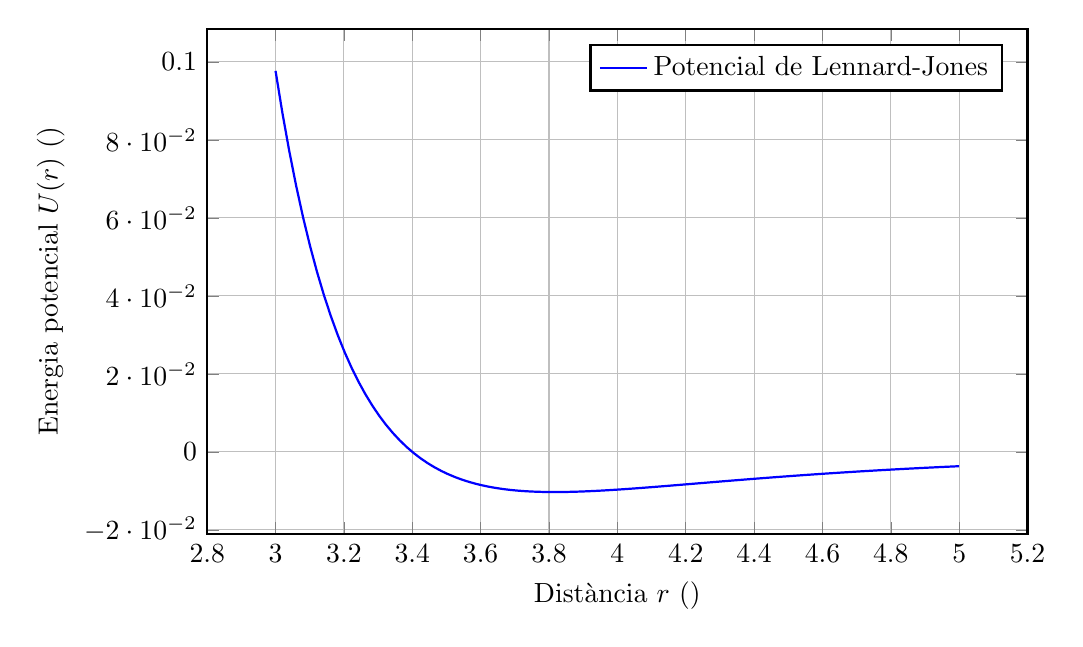
\begin{tikzpicture}
        \begin{axis}[
            width=12cm, height=8cm,
            xlabel={Distància \( r \) (\si{\angstrom})},
            ylabel={Energia potencial \( U(r) \) (\si{\electronvolt})},
            domain=3:5,
            samples=100,
            grid=major,
            thick,
            legend pos=north east
        ]
        \addplot[blue, thick] {4*0.0103*((3.4/x)^12 - (3.4/x)^6)};
        \legend{Potencial de Lennard-Jones}
        \end{axis}
    \end{tikzpicture}
    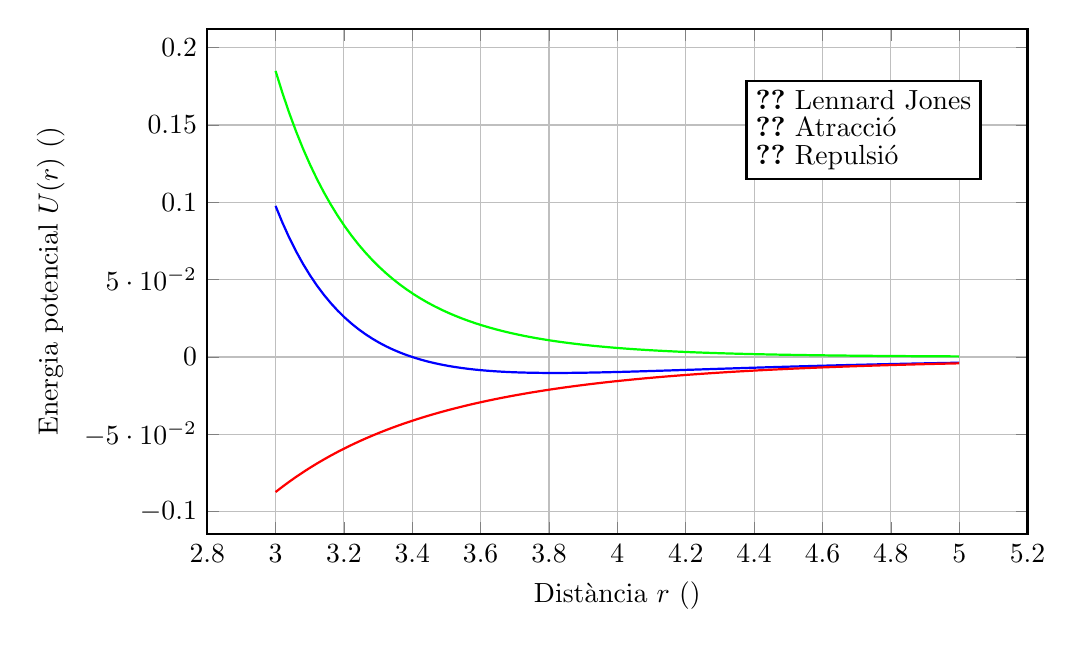
\begin{tikzpicture}
      \begin{axis}[
          width=12cm, height=8cm,
          xlabel={Distància \( r \) (\si{\angstrom})},
          ylabel={Energia potencial \( U(r) \) (\si{\electronvolt})},
          domain=3:5,
          samples=100,
          grid=major,
          thick,
          legend pos=north east
      ]
      \addplot[blue, thick] {4*0.0103*((3.4/x)^12 - (3.4/x)^6)};
      \label{LJ}
      \addplot[red, thick] {4*0.0103*(- (3.4/x)^6)};
      \label{att}
      \addplot[green, thick] {4*0.0103*((3.4/x)^12) };
      \label{rep}
      \node [draw,fill=white] at (rel axis cs: 0.8,0.8) {\shortstack[l]{
              \ref{LJ} Lennard Jones \\
              \ref{att} Atracció \\
              \ref{rep} Repulsió}};
      \end{axis}
  \end{tikzpicture}
    \caption{Potencial de Lennard-Jones amb valors típics (\(\varepsilon = \qty{0.010}{\electronvolt}\), \(\sigma = \qty{3.4}{\angstrom}\)). L'energia potencial disminueix inicialment fins a un mínim, corresponent a la distància d'equilibri on la interacció és més estable. Quan les molècules s'acosten massa, la repulsió electrònica domina i l'energia potencial augmenta ràpidament.}
\end{figure}





%\begin{exr}
Perquè \ch{CO2} i \ch{O2} tenen una desviació negativa respecte al comportament del gas ideal a pressions i temperatures moderades, mentres que l'He i el \ch{H2} presenten una deviació positiva en les mateixes condicions?
\end{exr}
\lct{
    Els gasos \ch{CO2} i \ch{O2} presenten una desviació negativa respecte al comportament ideal perquè tenen interaccions intermoleculars atractives significatives. Aquestes forces atractives fan que, a pressions i temperatures moderades, les molècules s'acostin més del que prediu l'equació del gas ideal, reduint així el volum efectiu i fent que el factor de compressibilitat \( z = \frac{PV}{RT} \) sigui menor que 1.

D'altra banda, els gasos com l'heli (\ch{He}) i l'hidrogen (\ch{H2}) presenten una desviació positiva perquè tenen interaccions intermoleculars molt febles i, a mesura que augmenta la pressió, dominen els efectes de repulsió a causa del volum finit de les molècules. Això fa que el gas ocupi un volum lleugerament superior al que prediu el model ideal, fent que \( z > 1 \) en aquestes condicions.
}

\newpage
\section{Exercicis}
\begin{exr}
    Un conductor comprova la pressió dels pneumàtics pel matí aviat, quan la temperatura és de 15\si\degreeCelsius, i és de 1.3$\times$10$^5$ Pa. Al migdia la temperatura és 15 graus més elevada. Quina és la pressió dels pneumàtics ara?.
    \end{exr}
	
\begin{exr}{}
        Dalt de l'Everest, la pressió atmosfèrica és de 0,33 atm i la temperatura de 50 sota zero. Quina és la densitat de l'aire si en CN és de 1.29\si{\gram\per\deci\meter\tothe{3}}?.
        \end{exr}
    \lct{


Sabem que la densitat de l'aire en condicions normals (CN) és:

\[
\rho_{\text{CN}} = \SI{1.29}{\gram\per\deci\meter\cubed}
\]

Les condicions a dalt de l’Everest són:

\begin{itemize}
    \item Pressió atmosfèrica: \( P = \SI{0.33}{\atm} \)
    \item Temperatura: \( T = \SI{-50}{\celsius} = \SI{223}{\kelvin} \)
    \item Condicions normals (CN):
    \begin{itemize}
        \item Pressió normal: \( P_{\text{CN}} = \SI{1}{\atm} \)
        \item Temperatura normal: \( T_{\text{CN}} = \SI{273}{\kelvin} \)
    \end{itemize}
\end{itemize}

Sabem que la densitat d'un gas està relacionada amb la pressió i la temperatura segons l'expressió:

\[
\frac{\rho}{\rho_{\text{CN}}} = \frac{P}{P_{\text{CN}}} \times \frac{T_{\text{CN}}}{T}
\]

Aïllant \( \rho \):

\[
\rho = \rho_{\text{CN}} \times \frac{P}{P_{\text{CN}}} \times \frac{T_{\text{CN}}}{T}
\]

Substituïm els valors donats:

\[
\rho = (\SI{1.29}{\gram\per\deci\meter\cubed}) \times \frac{\SI{0.33}{\atm}}{\SI{1}{\atm}} \times \frac{\SI{273}{\kelvin}}{\SI{223}{\kelvin}}=\SI{0.52}{\gram\per\deci\meter\cubed}
\]

    }
	
\begin{exr}
    Calcular el volum molar d'un gas ideal a condicions normals (1 atm i 0\si\degreeCelsius).
    \end{exr}

\lct{

    
    \subsection*{Dades donades}
    Les condicions normals (CN) per a un gas ideal són:
    
    \begin{itemize}
        \item Pressió: \( P = \SI{1}{\atm} \)
        \item Temperatura: \( T = \SI{0}{\celsius} = \SI{273.15}{\kelvin} \)
        \item Constant dels gasos: \( R = \SI{0.0821}{\liter\atm\per\mole\per\kelvin} \)
    \end{itemize}
    
    \subsection*{Aplicació de l'equació dels gasos ideals}
    L'equació dels gasos ideals és:
    
    \[
    PV = nRT
    \]
    
    Aïllem el volum molar \( V_m \), considerant \( n = 1 \) mol:
    
    \[
    V_m = \frac{RT}{P}
    \]
    
    \subsection*{Càlcul del volum molar}
    Substituïm les dades:
    
    \[
    V_m = \frac{(\SI{0.0821}{\liter\atm\per\mole\per\kelvin}) \times (\SI{273.15}{\kelvin})}{\SI{1}{\atm}}
    \]
    
    \[
    V_m = \frac{\SI{22.414}{\liter\atm\per\mole}}{\SI{1}{\atm}}
    \]
    
    \[
    V_m \approx \SI{22.4}{\liter\per\mole}
    \]
    
    \subsection*{Conclusió}
    El volum molar d’un gas ideal en **condicions normals** és **\(\SI{22.4}{\liter\per\mole}\)**.
    
    

}
\begin{exr}
    Quant gas hi ha en una mostra de volum \qty{0.5}{\deci\meter\tothe{3}}, a \qty{80}{\degC} i \qty{800}{\torr} de pressió?
    \end{exr}

\begin{exr}
Pots calcular el volum ocupat per molècula en un gas ideal a CN?. Es troben dues molècules molt freqüentment en un gas a baixa pressió?
\end{exr}
\begin{exr}{}
        Si a CN la densitat d'un gas ideal és de \qty{2.62}{\gram\per\deci\meter\tothe{3}}, quina és la seva massa molar? i quina densitat tindrà a 300 K i \qty{2.4e5}{\pascal} 2.4$\times$10$^5$ Pa?
        \end{exr}


        

\begin{exr}{}
Què passa segons l'Equació de van der Waals si la pressió es fa propera a zero o bé la temperatura es fa molt gran per a un gas real?   La figura mostra el factor de compressibilitat per a un mateix gas a diferents temperatures
\begin{center}        \includegraphics[scale=1.0]{FactorCompressT.png}
\end{center}
\end{exr}

\begin{exr}{Comparativa TCG per a \ch{H2} i \ch{He}}
Es prepara una mescla de gasos d'hidrogen (\ch{H2}) i heli (\ch{He}) tal que les molècules de cada gas produeixin el mateix nombre de col·lisions amb la paret per unitat de temps. Determinem quin gas té la concentració més alta.
\end{exr}
\lct{
\textbf{Consideració com a gasos ideals}

L'energia cinètica translacional d'un mol de gas és 
\[\left<E_c\right>=N_0 \frac{m <c^2>}{2}=\frac{3}{2} RT\]
on $M=N_0m$ és la massa molecular del gas en \si{\kilogram\per\mole}. 

Per tant, la velocitat quadràtica mitjana és:

\begin{equation}
    c_{\text{rms}} = \sqrt{\frac{3RT}{M}}
\end{equation}
Com que la taxa de col·lisions amb la paret és proporcional a $n v_{\text{rms}}$, imposem la condició d'igualtat:
\begin{equation}
    n_{\ch{H2}} \cdot \sqrt{\frac{3RT}{M_{\ch{H2}}}} = n_{\ch{He}} \cdot \sqrt{\frac{3RT}{M_{\ch{He}}}}
    \label{Eq:igualtat}
\end{equation}

A l'Eq. \ref{Eq:igualtat} hem usat que el nombre de col·lisions és proporcional al producte del nombre de molècules per la velocitat promig a la que es mouen. Per a entendre-ho, imaginem un cas simple de tres pilotes que es mouen a 10 m/s en línia recta i fan rebots entre dues parets d'una habitació. Si l'habitació fa 10 metres de llarg, en 10 segons cada pilota haurà tocat les parets 10 cops. Per tant, el nombre de xocs haurà estat 30.
Si enlloc de 3 pilotes en tinguéssim 10 que es mouen a 3 metres per segon, haurien tocat les parets també 30 cops (cada pilota, en 10 segons, hauria recorregut 30 metres, i per tant hauria xocat 3 cops contra les parets; com que tenim 10 pilotes, el nombre total de xocs és 30).

Substituint masses moleculars $M_{\ch{H2}} = 2$ g/mol i $M_{\ch{He}} = 4$ g/mol a l'Eq. \ref{Eq:igualtat}:
\begin{equation}
    n_{\ch{H2}} \cdot \sqrt{\frac{1}{2}} = n_{\ch{He}} \cdot \sqrt{\frac{1}{4}}
\end{equation}
\begin{equation}
    n_{\ch{H2}} \cdot \frac{1}{\sqrt{2}} = n_{\ch{He}} \cdot \frac{1}{2}
\end{equation}
Resolent per $n_{\ch{H2}}$:
\begin{equation}
    n_{\ch{H2}} = \frac{n_{\ch{He}}}{\sqrt{2}}
\end{equation}
Per tant, la concentració de $\ch{H2}$ ha de ser més baixa que la de $\ch{He}$.
És a dir, si volem igualar les vegades que xoquen contra les parets d'un volum les molècules d'He i d'H2, hem de plantejar l'expressió d'igualtat de l'Eq. \ref{Eq:igualtat} on la partícula amb més massa, pel fet d'anar més lenta, necessitarà més partícules en moviment, és a dir, més concentració.

%\\[10pt]
\textbf{Consideració com a gasos no ideals}

Si considerem gasos reals, hem de corregir la velocitat mitjana tenint en compte el factor de compressibilitat $Z$:
\begin{equation}
    v_{\text{rms}} = \sqrt{\frac{3ZRT}{M}}
\end{equation}
Ara, l'Eq. \ref{Eq:igualtat} es transforma en:
\[
    n_{\ch{H2}} \cdot \sqrt{\frac{3Z_{\ch{H2}}RT}{M_{\ch{H2}}}} = n_{\ch{He}} \cdot \sqrt{\frac{3Z_{\ch{He}}RT}{M_{\ch{He}}}}
\]
d'on
\[
    \frac{n_{\ch{H2}}}{n_{\ch{He}}}=\sqrt{\frac{\frac{3Z_{\ch{He}}RT}{M_{\ch{He}}}}{\frac{3Z_{\ch{H2}}RT}{M_{\ch{H2}}}}}
    =\sqrt{\frac{Z_{\ch{He}}M_{\ch{H2}}}{Z_{\ch{H2}}M_{\ch{He}}}}
\]
A pressions altes, $Z_{\ch{H2}} > Z_{\ch{He}}$ per les interaccions intermoleculars més fortes d'hidrogen (veure la Fig. Gasos-\ref{Gasos-fig:FactorCompress}), la qual cosa encara reforça més la diferència entre les concentracions de les dues expècies químiques. 
}


\begin{qst}
La composició percentual, en massa, de l'aire sec al nivell del mar és, aproximadament, \ch{N2}/\ch{O2}/\ch{Ar}=75.5/23.2/1.3. 
Quina és la pressió parcial de cada component quan la pressió total és 1.20 atm?
(extret de \cite{Atkins2018}).
\end{qst}
\lct{
En 100gr d'aire tindrem 75.5, 23.2 i 1.3 gr de \ch{N2}, \ch{O2} i \ch{Ar}, respectivament. Podem calcular la seva fracció molar calculant el número de mols de cadascun i dividint pel total. Després, només cal multiplicar per la pressió corresponent i sabrem la pressió parcial de cada component:

\[n_{\ch{N2}}=75.5 \cancel{g} \cdot \frac{1 mol}{28.02 \cancel{g}}=2.69 mol\]
\[n_{\ch{O2}}=23.2 \cancel{g} \cdot \frac{1 mol}{32.00 \cancel{g}}=0.725 mol\]
\[n_{\ch{Ar}}=1.3 \cancel{g} \cdot \frac{1 mol}{39.95 \cancel{g}}=0.033 mol\]

    \begin{tabular}{cccc}
      \hline
        & \ch{N2} & \ch{O2} & \ch{Ar} \\
      \hline
Fracció molar &	0.780 & 0.210 & 0.0096\\
Pressió parcial (nivell del mar)/atm & 0.780 & 0.210 & 0.0096\\
Pressió parcial ($P_T=1.20$atm))/atm & 0.936 & 0.252 & 0.012\\
      \hline
    \end{tabular}

}
 % Dalton
\begin{exr}{Fracció metà en una mescla}
Una barreja de metà \ch{CH4} i d'acetilè \ch{C2H2} ocupava un cert volum a una pressió total de 63 mmHg. La mostra es va cremar a \ch{CO2} i \ch{H2O}. Se'n va recollir el \ch{CO2} en el mateix volum inicial i la mateixa temperatura inicial, i es va veure que la seva pressió era de 96 mmHg. Quina era la fracció de metà a la mescla de gasos inicials?
\end{exr}
\lct{

    \textbf{OPCIÓ 1:\\}
Definim $x$ com la fracció molar de metà (\ch{CH4}) i $y$ com la fracció molar d’acetilè (\ch{C2H2}):  
        \[
        x + y = 1
        \]
   
    Les reaccions de combustió són:
    \begin{eqnarray}
        \ch{CH4 + 2 O2 -> CO2 + 2 H2O}  \label{Eq:meta} \\
        \ch{C2H2 + 5/2 O2 -> 2 CO2 + H2O}  \label{Eq:acetile}
    \end{eqnarray}
on veiem que 1 mol de \ch{CH4} produeix 1 mol de \ch{CO2} i que 1 mol de \ch{C2H2} produeix 2 mols de \ch{CO2}. Si tenim un nombre total de mols $n$, llavors:
    \begin{itemize}
        \item Mols de metà: $xn$
        \item Mols d'acetilè: $yn$
    \end{itemize}
    
    Els mols de \ch{CO2} formats són:
    \[
    n_{\ch{CO2}} = xn + 2yn
    \]
     
    Com que el volum i la temperatura es mantenen constants, segons la llei dels gasos ideals la pressió és directament proporcional als mols:
        \[
    P_{\ch{CO2}} = (xn + 2yn) \cdot \frac{P_{\text{total}}}{n}
    \]
    
    Substituint els valors donats:
        \[
    96 = (x + 2y) \cdot 63
    \]
    
   d'on
    \[
    x + 2y = \frac{32}{21}
    \]
    
   Ara ja podem resoldre el sistema:
        \begin{align}
        x + y &= 1 \\
        x + 2y &= \frac{32}{21}
    \end{align}
     i obtenim   
    \[
    x = 1 - \frac{11}{21} = \frac{10}{21}
    \]
    
    Per tant, la fracció de metà en la mescla inicial és:
        \[
    \frac{10}{21} \approx 0.476 \quad \text{o} \quad 47.6\%
    \]

    \textbf{OPCIÓ 2:\\}
Definim les pressions parcials inicials com $P_{\ch{CH4}}^i=x$ i $P_{\ch{C2H2}}^i=y$. Segons les Equacions \ref{Eq:meta} i \ref{Eq:acetile}, les pressions finals seran $P_{\ch{CH4}}^f=x$ i $P_{\ch{C2H2}}^f=2y$. Sabent que la pressió total inicial és \qty{63}{\mmHg} i que la final és \qty{96}{\mmHg}, obtenim el sistema:

\[
\systeme{x+y=63,x+2y=96}
\]
Solucionant-lo, obtenim que $x=\qty{30}{\mmHg}$ i $y=\qty{33}{\mmHg}$ 
que impliquen fraccions molars inicial de $\chi_{\ch{CH4}}^i=30/63=0.476$ i $\chi_{\ch{C2H2}}^i=33/63=0.523$.

Notar que usar la llei dels gasos ideals i, per tant, observar que podem treballar indistintament amb nombre de mols o pressions parcials sempre que la reacció involcri gasos, simplifica la resolució de l'exercici.


}

\begin{exr}
    Un compost gasós que se sap que conté només carboni, hidrogen i nitrogen es barreja amb el volum d'oxigen exactament necessari per a la seva combustió completa a \ch{CO2}, \ch{H20} i \ch{N2}. La combustió de 9 volums de la mescla gasosa produeix 4 volums de \ch{CO2}, 6 volums de vapor d'aigua i 2 volums de \ch{N2}, tots a la mateixa temperatura i pressió.

    Quants volums d'oxigen es necessiten per a la combustió? Quina és la fórmula molecular del compost?
\end{exr}

\lct{

El compost gasós conté carboni (C), hidrogen (H) i nitrogen (N). Es barreja amb oxigen suficient per a la combustió completa, donant com a productes diòxid de carboni (\(\ch{CO2}\)), aigua (\(\ch{H2O}\)) i nitrogen molecular (\(\text{N}_2\)).

Es donen les següents dades:
\begin{itemize}
    \item Volum de la mescla gasosa: 9 volums
    \item Volum de \(\ch{CO2}\) produït: 4 volums
    \item Volum de \(\ch{H2O}\) produït: 6 volums
    \item Volum de \(\text{N}_2\) produït: 2 volums
\end{itemize}

Sigui la fórmula del compost:
\[
C_xH_yN_z
\]

L'equació de combustió és:
\[
C_xH_yN_z + \ch{O2} \rightarrow a C\ch{O2} + b \ch{H2O} + c N_2
\]

Per la conservació dels àtoms:

- Carboni: \( x = a = 4 \Rightarrow x = 4 \)
- Hidrogen: \( y = 2b = 6 \Rightarrow y = 6 \)
- Nitrogen: \( z = 2c = 2 \Rightarrow z = 2 \)

Així, la fórmula del compost és:
\[
C_4H_6N_2
\]

Per trobar el volum d'oxigen utilitzat, considerem la combustió completa:

\[
C_4H_6N_2 + \ch{O2} \rightarrow 4 C\ch{O2} + 3 \ch{H2O} + N_2
\]

L'oxigen es consumeix en la formació de \(\ch{CO2}\) i \(\ch{H2O}\):

\[
\ch{O2} \text{ necessari} = \frac{(4 \times 2) + (3 \times 1)}{2} = \frac{8 + 3}{2} = 5.5 \text{ volums}
\]

Per tant, el volum d'oxigen necessari és **5.5 volums**.

}

\input{../Exercicis/ex_hidrogenacioEtile.tex}
\begin{exr}{Pressió parcial \ch{PCl5} en una mescla}
    Una mostra de \ch{PCl5}, que pesa \SI{2.69}{\gram}, es va col·locar en un flascó d'\SI{1.00}{\litre} i es va evaporar completament a una temperatura de \SI{250}{\celsius}. La pressió observada a aquesta temperatura va ser \SI{1.00}{\atm}. Existeix la possibilitat que una part del \ch{PCl5} s'hagi dissociat d'acord amb l'equació:

\begin{reaction}
PCl5(g) -> PCl3(g) + Cl2(g)
\end{reaction}

Quines són les pressions parcials del \ch{PCl5}, \ch{PCl3} i \ch{Cl2} en aquestes condicions experimentals? (Adaptat de \cite{mahan_quimica_1997})
\end{exr}
\lct{
    La solució d'aquest problema implica diverses etapes. Per determinar si s'ha dissociat una part del \ch{PCl5}, calculem primerament la pressió que s'hauria observat si no s'hagués dissociat el \ch{PCl5}. Això es pot calcular a partir del nombre de mols de \ch{PCl5} utilitzats, juntament amb el volum i la temperatura del flascó. Com que el pes molecular del \ch{PCl5} és \SI{208}{\gram\per\mole}, el nombre de mols de \ch{PCl5} inicialment presents en el flascó és:

\[
n = \SI{2.69}{\gram}\cdot \frac{1\si{\mole}}{\SI{208}{\gram}} = 0.0129\si{\mole}.
\]

La pressió corresponent a aquest nombre de mols seria:

\[
P = \frac{nRT}{V} = \frac{(0.0129\si{\mole})(\SI{0.082}{\liter\atm\per\mole\per\kelvin})(\SI{523.15}{\kelvin})}{\SI{1.00}{\liter}} = \SI{0.553}{\atm}.
\]

Com que la pressió observada és superior a aquesta, s'ha de produir certa dissociació del \ch{PCl5}. Aplicant la llei de les pressions parcials, podem escriure:

\begin{equation}
P_{\ch{PCl5}} + P_{\ch{PCl3}} + P_{\ch{Cl2}} = P_t = \SI{1.00}{\atm}.
\label{eq:daltonpcl}
\end{equation}

Ara observem que:


Atès que es produeix un mol de \ch{PCl3} i un mol de \ch{Cl2} per cada mol de \ch{PCl5} dissociat,
\[
P_{\ch{Cl2}} = P_{\ch{PCl3}}, \quad P_{\ch{PCl5}} = \SI{0.553}{\atm} - P_{\ch{Cl2}}.
\]
i podem reescriure l'Equació \ref{eq:daltonpcl} com:

\[
\SI{0.553}{\atm} - P_{\ch{Cl2}} + P_{\ch{Cl2}} + P_{\ch{Cl2}} = \SI{1.00}{\atm}.
\]

Resolent, obtenim:

\[
P_{\ch{Cl2}} = \SI{0.447}{\atm},
\]

i

\[
P_{\ch{PCl3}} = \SI{0.447}{\atm}, \quad P_{\ch{PCl5}} = \SI{0.106}{\atm}.
\]
}

\begin{exr}{Relació $\frac{C_P}{C_V}$}
Perquè hi ha diferències entre els quocients de capacitat calorífica ($C_P/C_V$) de gasos monoatòmics respecte els diatòmics? (Adona't que si un gas monoatòmic ideal, pel fet d'estar només augmentant la seva energia cinètica translacional té una $C_V=\frac{3}{2}R$, es pot entendre que per a cada component (eix) necessita $\frac{1}{2}R$)
\end{exr}
\lct{
    Els quocients de la capacitat calorífica dels gasos diatòmics són molt menors que 1,67, i hem d'esbrinar la raó d'aquestes desviacions.

    Primerament, notem que $C_V$, la capacitat calorífica deguda al moviment de translació de les molècules, és igual a $\frac{3}{2}R$, i que hi ha tres components independents de velocitat associats amb el moviment de translació. Per tant, podem inferir que cadascun dels tres moviments de translació independents contribueix amb $\frac{1}{2}R$ a la capacitat calorífica molar. Sobre aquesta base, podríem esperar que, si algun altre tipus de moviment fos accessible a les molècules de gas, hi hauria més contribucions a la capacitat molar i aquestes entrarien en unitats de $\frac{1}{2}R$.
    
   A més de tenir els tres moviments de translació, una molècula diatòmica pot rotar al voltant del seu centre de massa segons dos modes mútuament perpendiculars i independents. Assignant $\frac{1}{2}R$ com la contribució de cadascun d'aquests moviments a la capacitat calorífica, tenim:
    
    \[
    C_V = \underbrace{\frac{3}{2}R}_{\text{traslació}} + \underbrace{\frac{1}{2}R + \frac{1}{2}R}_{\text{rotació}} = \frac{5}{2}R,
    \]
    
    \[
    C_P = C_V + R = \frac{7}{2}R,
    \]
    
    \[
    \frac{C_P}{C_V} = \frac{\frac{7}{2}R}{\frac{5}{2}R} = \frac{7}{5} = 1,40.
    \]
}

\begin{exr}
Qui es mou més ràpid, una molècula d'oxigen o una de nitrogen en dues mostres d'aquests gasos a la mateixa temperatura? Pots explicar perquè la pressió és independent de la natura de les molècules?
\end{exr}

\begin{exr}{}
Calcula la velocitat mitjana de les molècules d'hidrògen a 25\si\degreeCelsius.
\end{exr}
\lct{
La velocitat mitjana de les molècules d'un gas es pot calcular a partir de la distribució de Maxwell-Boltzmann. Utilitzant la distribució de Maxwell com a distribució de probabilitats, es pot determinar la velocitat mitjana molecular en una mostra de gasos:

\begin{equation*}
    \langle v \rangle = \int_{-\infty}^{\infty} v f(v) dv
\end{equation*}

Substituint la funció de distribució de Maxwell-Boltzmann:

\begin{equation*}
    \langle v \rangle = \int_{-\infty}^{\infty} v \cdot 4\pi \left(\frac{m}{2\pi k_B T}\right)^{\frac{3}{2}} v^2 \exp{\left(-\frac{m v^2}{2 k_B T} \right)} dv
\end{equation*}

\noindent Aplicant la següent integral coneguda de les taules d'integrals:

\begin{equation*}
    \int_0^{\infty} x^{2n+1} e^{-a x^2} dx = \frac{n!}{2 a^{n+1}}
\end{equation*}
i agafant $n=1$, s'obté:

\begin{equation*}
    \langle v \rangle = 4\pi \left(\frac{m}{2\pi k_B T}\right)^{\frac{3}{2}} \cdot \frac{1}{2} \left(\frac{m}{2 k_B T}\right)^{-2}
\end{equation*}

Finalment, simplificant,

\begin{equation}
    \langle v \rangle = \sqrt{\frac{8 k_B T}{\pi m}}
    \label{eq:velocitatMitjana}
\end{equation}

Substituint les dades a l'Eq. \ref{eq:velocitatMitjana}::
\begin{equation}
    R = 8.314 \text{ J/mol·K}, \quad T = 298 \text{ K}, \quad M = 2.016 \times 10^{-3} \text{ kg/mol}
\end{equation}
\begin{equation}
    v_{mitjana} = \sqrt{\frac{8 \times 8.314 \times 298}{\pi \times 2.016 \times 10^{-3}}}
\end{equation}
\begin{equation}
    v_{mitjana} \approx 1.57 \times 10^3 \text{ m/s}
\end{equation}
}

\begin{exr}
Considerant que no es comporta idealment, calcula la temperatura de \qty{10}{\mole} de monòxid de carboni (\ch{CO}) sotmesos a una pressió de \qty{5}{\kilo\pascal} en un volum de \qty{2}{\meter\tothe{3}}.
\end{exr}
\lct{
    L'equació de Van der Waals per gasos reals és:

    \[
    \left( P + \frac{n^2 a}{V^2} \right) (V - nb) = nRT
    \]
    
on $a$ i $b$ són constants que depenen de la naturalesa del gas. En el nostre cas:

\begin{itemize}
    \item Nombre de mols: \( n = 10 \) mol  
    \item Pressió: \( P = \qty{5}{\kilo\pascal} \cdot \frac{\qty{1}{\atm}}{\qty{101.325}{\kPa}} = \qty{0.0493}{\atm} \)  
    \item Volum: \( V = \qty{2}{\meter\tothe{3}} = \qty{2000}{\liter} \)  
    \item Constants de Van der Waals per \ch{CO}:
    \begin{itemize}
        \item \( a = \qty{1.4850}{\liter\squared\atm\per\mole\squared} \)
        \item \( b = \qty{0.03985}{\liter\per\mole} \)
    \end{itemize}
    \item Constant dels gasos: \( R = \qty{0.0821}{\liter\atm\per\mole\per\kelvin} \)
\end{itemize}

Calculem el terme de correcció de la pressió:

\[
    P + \frac{a n^2}{V^2} = 0.0493+\frac{(1.4850)(10)^2}{(2000)^2} = \qty{0.0493}{\atm}
\]


Calculem el volum corregit:

\[
V - nb = 2000 - (10 \times 0.03985) = 2000 - 0.3985 = \qty{1999.6}{\liter}
\]

Es pot veure com l'efecte de la no idealitat en aquest gas és molt reduït.  
Substituïm a l'equació:

\[
(0.0493)(1999.6) = (10)(0.0821)T
\]


\[
T = \frac{98.57}{0.821} = \qty{120}{\kelvin}
\]
}

\begin{exr}
Perquè \ch{CO2} i \ch{O2} tenen una desviació negativa respecte al comportament del gas ideal a pressions i temperatures moderades, mentres que l'He i el \ch{H2} presenten una deviació positiva en les mateixes condicions?
\end{exr}
\lct{
    Els gasos \ch{CO2} i \ch{O2} presenten una desviació negativa respecte al comportament ideal perquè tenen interaccions intermoleculars atractives significatives. Aquestes forces atractives fan que, a pressions i temperatures moderades, les molècules s'acostin més del que prediu l'equació del gas ideal, reduint així el volum efectiu i fent que el factor de compressibilitat \( z = \frac{PV}{RT} \) sigui menor que 1.

D'altra banda, els gasos com l'heli (\ch{He}) i l'hidrogen (\ch{H2}) presenten una desviació positiva perquè tenen interaccions intermoleculars molt febles i, a mesura que augmenta la pressió, dominen els efectes de repulsió a causa del volum finit de les molècules. Això fa que el gas ocupi un volum lleugerament superior al que prediu el model ideal, fent que \( z > 1 \) en aquestes condicions.
}
\begin{exr}{Airbag}
    Els coixins de seguretat ({\em airbag}) dels cotxes s'inflen mitjançant una sèrie de reaccions químiques ràpides que produeixen gas en menys de \qty{0.04}{\second}. En les seves primeres versions, la reacció es basava en la descomposició de \ch{NaN3} (extremadament tòxic), seguida de dues reaccions addicionals per neutralitzar els subproductes perillosos. Les equacions químiques d'aquest procés són:  
 
    \begin{reactions}
        2 NaN3 &-> 2 Na + 3 N2 (g) "\label{reac:nan3}"\\
        10 Na + 2 KNO3 &-> K2O + 5 Na2O + N2 (g) "\label{reac:na}"\\
        K2O + Na2O + 2 SiO2 &-> K2SiO3 + Na2SiO3
    \end{reactions}

Un coixí de seguretat de conductor té un volum aproximat de \qty{65}{\liter} i la pressió final dins del coixí és de \qty{1.35}{\atm}. La temperatura dins del coixí just després de la reacció és \qty{300}{\celsius} (\qty{573}{\kelvin}). Suposem que s'utilitzen \qty{65}{\gram} de \ch{NaN3}.  

 
\begin{enumerate}
    \item Quina quantitat de nitrogen gas (\ch{N2}) es genera en mols només en la primera reacció?
    \item Quin volum ocuparà aquest gas dins del coixí de seguretat segons la llei dels gasos ideals? És suficient aquest volum per inflar completament el coixí de seguretat?
    \item Si considerem també la segona reacció, que genera més nitrogen gas, com afectaria això el volum total de gas produït?
    \item Quan el gas s'expandeix a l'exterior a través dels orificis del coixí, la seva pressió baixa de \qty{1.35}{\atm} a \qty{1.00}{\atm}. Quin percentatge de reducció de temperatura es produeix durant aquesta expansió?
\end{enumerate}
(Adaptat de \cite{bowers_understanding_2014}).
\end{exr}

\lct{
     \begin{enumerate}
    \item Quantitat de nitrogen gas (\ch{N2}) generada a R\ref{reac:nan3}:
    
    La reacció de descomposició de \ch{NaN3} és:  
    
    \begin{equation*}
        \ch{2 NaN3 -> 2 Na + 3 N2 (g)}
    \end{equation*}
    
    Primer, calculem el nombre de mols de \ch{NaN3} disponibles:  
    
    \begin{equation}
        n_{\ch{NaN3}} = \frac{\qty{65}{\gram}}{\qty{65.019}{\gram\per\mol}} = \qty{1.00}{\mol}
    \end{equation}
    
    De l'estequiometria de la reacció, per cada \qty{2}{\mol} de \ch{NaN3}, es formen \qty{3}{\mol} de \ch{N2}:  
    
    \begin{equation}
        n_{\ch{N2}} = \qty{1.00}{\mol} \times \frac{3}{2} = \qty{1.50}{\mol}
    \end{equation}
    
    \item Volum ocupat pel gas segons la llei dels gasos ideals:
    
    Utilitzem l'equació dels gasos ideals:  
    
    \begin{equation}
        V = \frac{nRT}{P}
    \end{equation}
    
    On:
    \begin{itemize}
        \item $n = \qty{1.50}{\mol}$
        \item $R = \qty{0.0821}{\liter\atm\per\mol\per\kelvin}$
        \item $T = \qty{573}{\kelvin}$
        \item $P = \qty{1.35}{\atm}$
    \end{itemize}
    
    \begin{equation}
        V = \frac{\qty{1.50}{\mol} \times \qty{0.0821}{\liter\atm\per\mol\per\kelvin} \times \qty{573}{\kelvin}}{\qty{1.35}{\atm}}= \qty{52.3}{\liter}
    \end{equation}
      
    El volum necessari per inflar el coixí de seguretat és d'uns \qty{65}{\liter}. Atès que només la primera reacció genera \qty{52.3}{\liter}, sembla que no és suficient. No obstant això, la segona reacció també genera gas \ch{N2}, augmentant el volum total.  
    
    \item Contribució de la segona reacció al volum total de gas:
    
    La reacció R\ref{reac:na} genera gas addicional:  
    
    \begin{equation}
        \ch{10 Na + 2 KNO3 -> K2O + 5 Na2O + N2 (g)}
    \end{equation}
    
    Cada \qty{10}{\mol} de Na reacciona per produir \qty{1}{\mol} de \ch{N2}. Sabem que la primera reacció va generar \qty{1.00}{\mol} de Na. Per tant, la segona reacció produeix:  
    
    \begin{equation}
        n_{\ch{N2,2}} = \qty{1.00}{\mol} \times \frac{1}{10} = \qty{0.10}{\mol}
    \end{equation}
    
    Afegint aquest nitrogen al total:  
    
    \begin{equation}
        n_{\ch{N2,\text{total}}} = \qty{1.50}{\mol} + \qty{0.10}{\mol} = \qty{1.60}{\mol}
    \end{equation}
    
    El nou volum total serà:  
    
    \begin{equation}
        V_{\text{total}} = \frac{\qty{1.60}{\mol} \times \qty{0.0821}{\liter\atm\per\mol\per\kelvin} \times \qty{573}{\kelvin}}{\qty{1.35}{\atm}} = \qty{55.7}{\liter}
    \end{equation}
    
    Aquest volum segueix estant lleugerament per sota del mínim requerit (\qty{65}{\liter}), però cal recordar que les reaccions són fortament exotèrmiques, la qual cosa elevarà la temperatura i, en conseqüència, augmentarà el volum de gas.
    
    \item Refredament del gas en expandir-se fora del coixí:
    
    Segons la llei de Gay-Lussac:
    
    \begin{equation}
        \frac{P_1}{T_1} = \frac{P_2}{T_2}
    \end{equation}
    
    On:
    \begin{itemize}
        \item $P_1 = \qty{1.35}{\atm}$, $T_1 = \qty{573}{\kelvin}$
        \item $P_2 = \qty{1.00}{\atm}$, $T_2$ és la temperatura final
    \end{itemize}
    
    \begin{equation}
        T_2 = T_1 \times \frac{P_2}{P_1}
 = \qty{573}{\kelvin} \times \frac{\qty{1.00}{\atm}}{\qty{1.35}{\atm}}
= \qty{424}{\kelvin}
    \end{equation}
    
    El percentatge de reducció de temperatura és:
    
    \begin{equation}
        \frac{T_1 - T_2}{T_1} \times 100 = \frac{\qty{573}{\kelvin} - \qty{424}{\kelvin}}{\qty{573}{\kelvin}} \times 100 = 25.9\%
    \end{equation}
    
    Així, la temperatura del gas disminueix aproximadament un \qty{26}{\percent} quan s'expandeix fora del coixí de seguretat, ajudant a evitar cremades als passatgers.
\end{enumerate}
}

\section{Codis}

\begin{lstlisting}[language=Matlab, caption={Codi Matlab per dibuixar una distribució de Maxwell-Boltzmann}]
    clc; clear; close all;
    
    % Definim constants
    kB = 1.38e-23;  % Constant de Boltzmann (J/K)
    T = 300;        % Temperatura en Kelvin
    m = 4.65e-26;   % Massa de la molècula (kg) (exemple: molècula de nitrogen)
    
    % Definim el rang de velocitats
    v = linspace(0, 2000, 1000);  % Rang de velocitats (m/s)
    
    % Funció de distribució de Maxwell-Boltzmann
    f_v = ( (m / (2 * pi * kB * T))^(3/2) ) * 4 * pi * v.^2 .* exp(-m * v.^2 / (2 * kB * T));
    
    % Representació gràfica de la distribució
    figure;
    plot(v, f_v, 'b', 'LineWidth', 2);
    xlabel('Velocitat (m/s)');
    ylabel('Densitat de probabilitat f(v)');
    title('Distribució de Maxwell-Boltzmann');
    grid on;
    
    % Càlcul de la velocitat més probable, la velocitat mitjana i la velocitat quadràtica mitjana
    v_mp = sqrt(2 * kB * T / m);  % Velocitat més probable
    v_mitjana = sqrt(8 * kB * T / (pi * m));  % Velocitat mitjana
    v_rms = sqrt(3 * kB * T / m);  % Velocitat quadràtica mitjana
    
    hold on;
    xline(v_mp, '--r', 'Velocitat més probable', 'LabelHorizontalAlignment', 'right');
    xline(v_mitjana, '--g', 'Velocitat mitjana', 'LabelHorizontalAlignment', 'right');
    xline(v_rms, '--m', 'Velocitat RMS', 'LabelHorizontalAlignment', 'right');
    legend('Distribució de Maxwell-Boltzmann', 'Velocitat més probable', 'Velocitat mitjana', 'Velocitat RMS');
    hold off;
    \end{lstlisting}
